\subsection{Interpolating Trajectories}
\label{sec::313_it}
As already shortly depicted in figure \ref{fig::31_pg}, we need to interpolate the trajectories that we obtain from the nonlinear model predictive control. This especially holds true for the feet, since the computed results do only consider the pendulums dynamic balance with respect to the x-, and the y-position, but not with respect to a robot that has to lift its feet along the z-axis. Furthermore, the feet's movement shall be executed such they stop moving when they are about to touch the ground. This constraint, and others, will be achieved by interpolating the feet trajectories with polynomials. In order to then match the center of mass trajectory's temporal resolution with the feet trajectories', we will upscale it under the already well known assumption of a linear inverted pendulum. The resulting trajectories are shown in figure \ref{fig::313_ip}, and will further be explained in the following. 
\begin{figure}[h]
	\centering
	\subcaptionbox{}%
	[.4\linewidth]{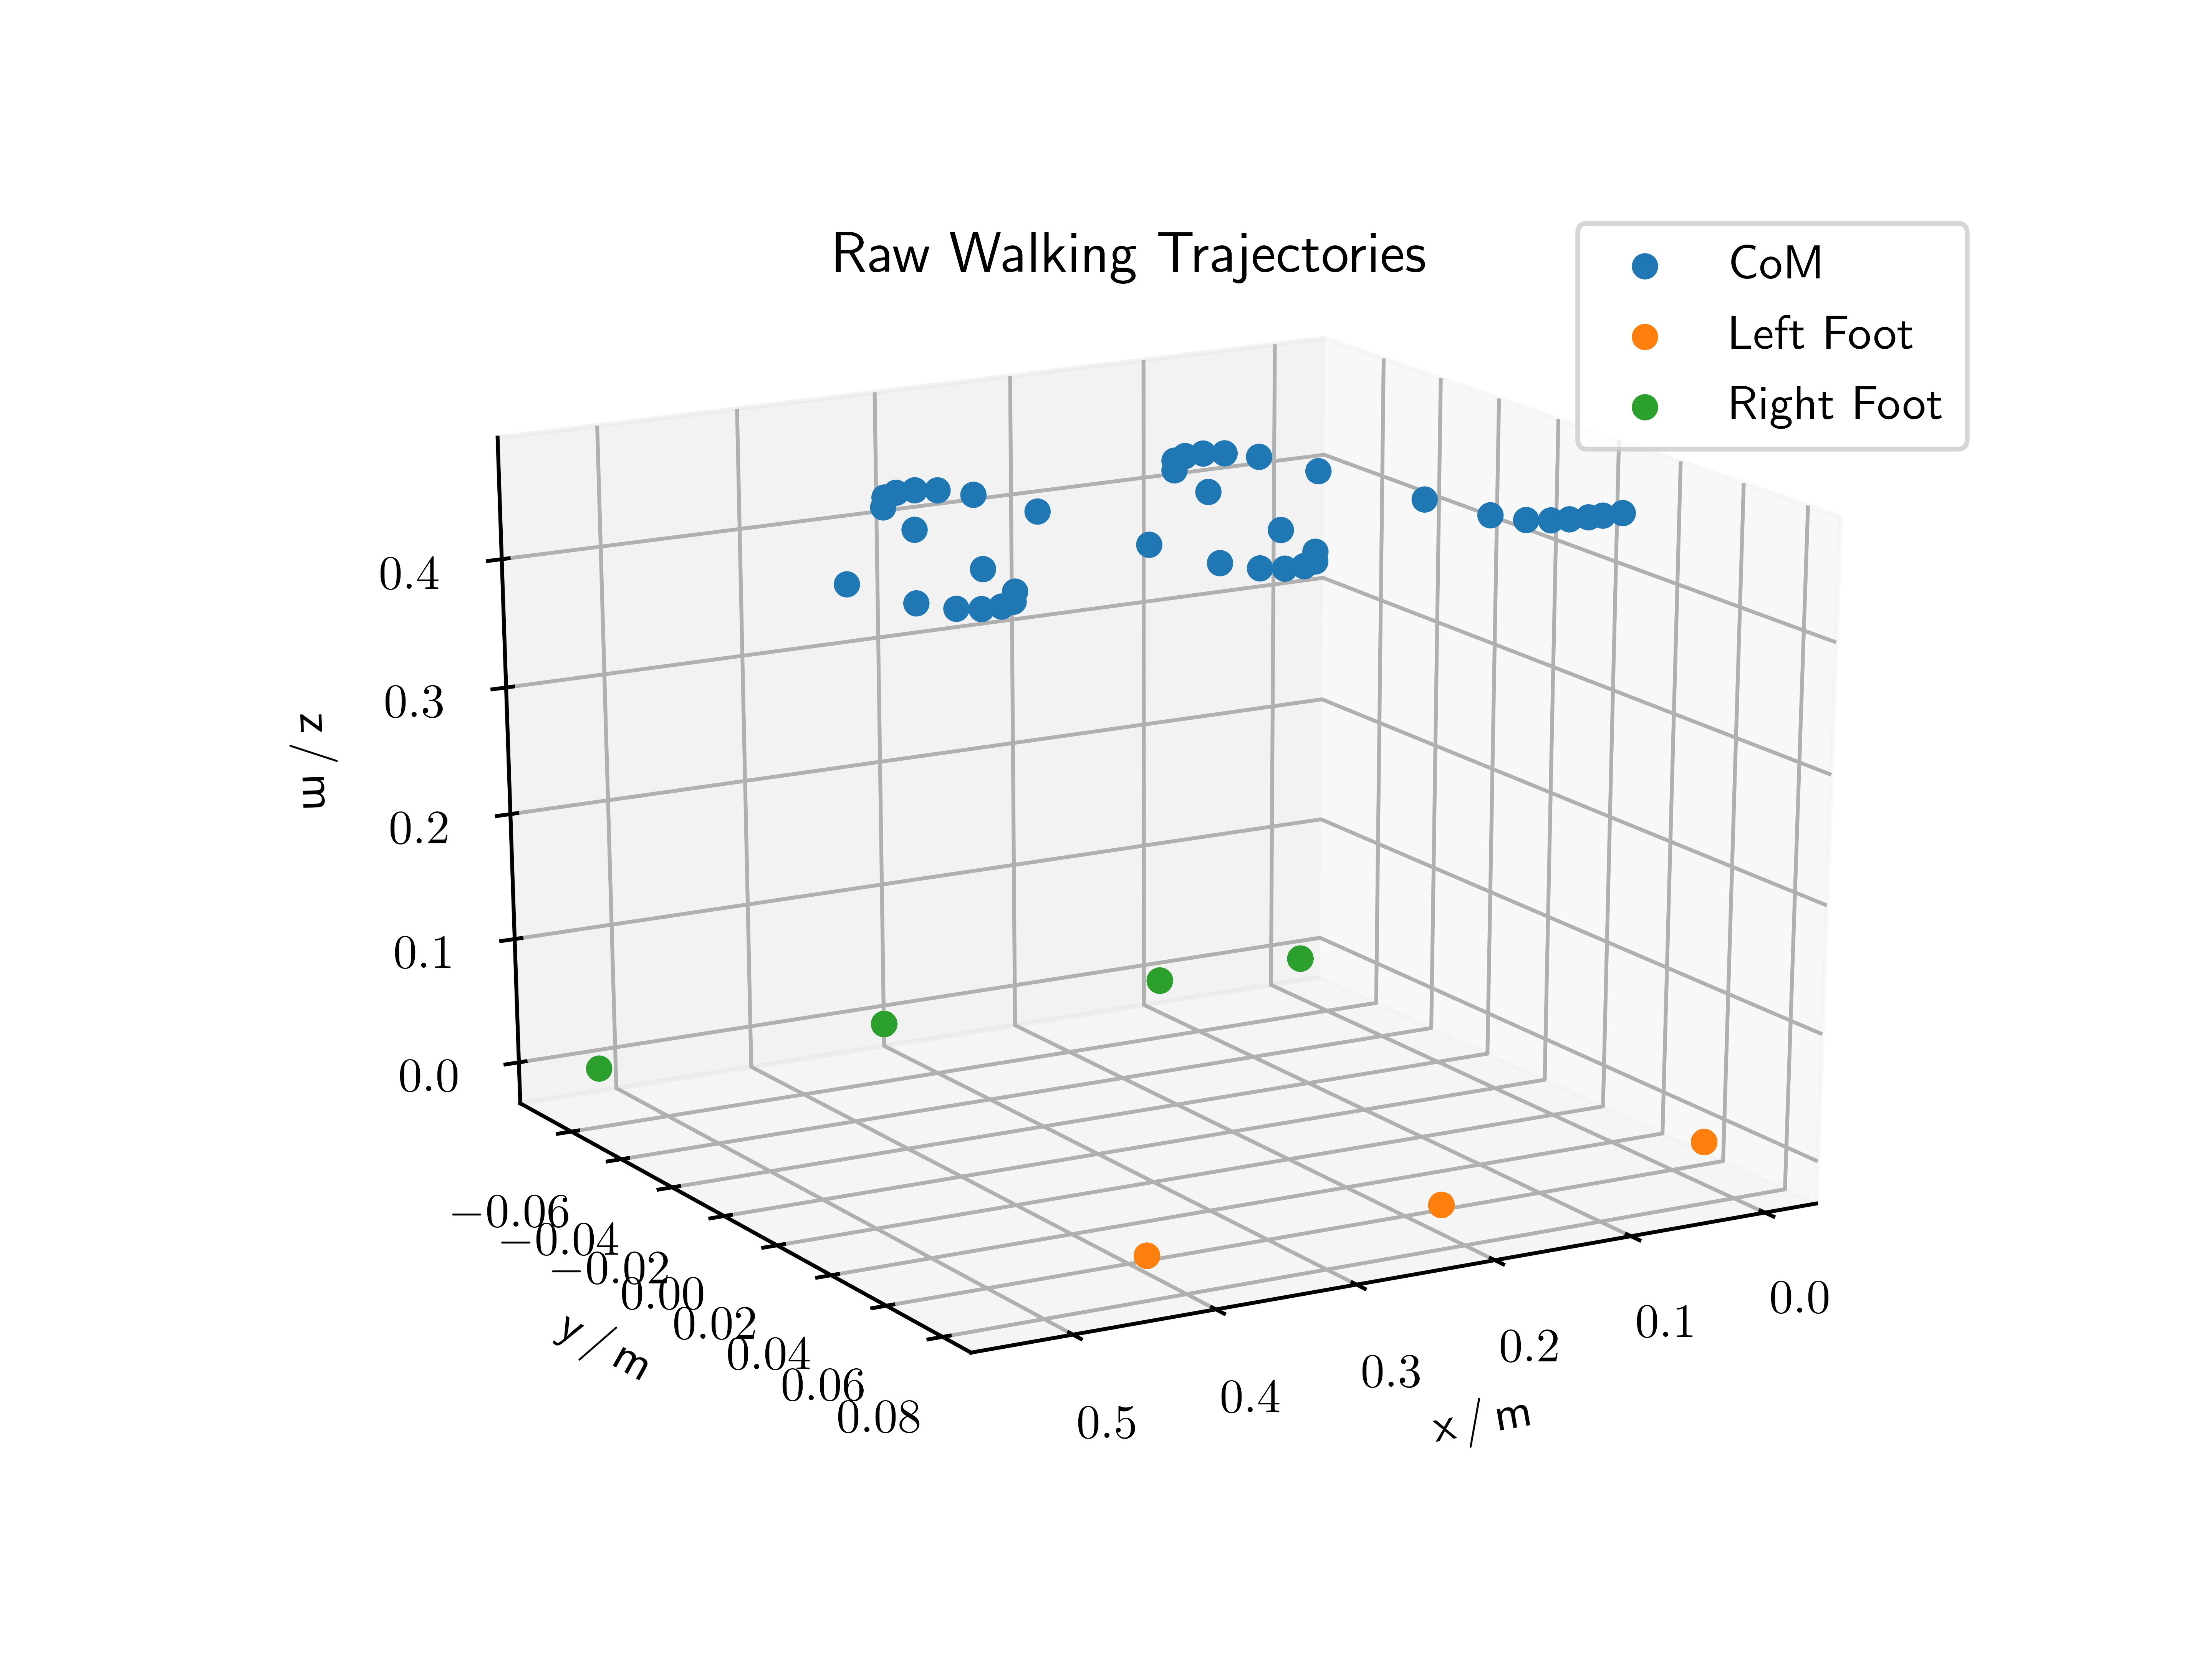
\includegraphics[scale=.4]{chapters/03_background/img/raw_results.png}}
	\subcaptionbox{}%
	[.4\linewidth]{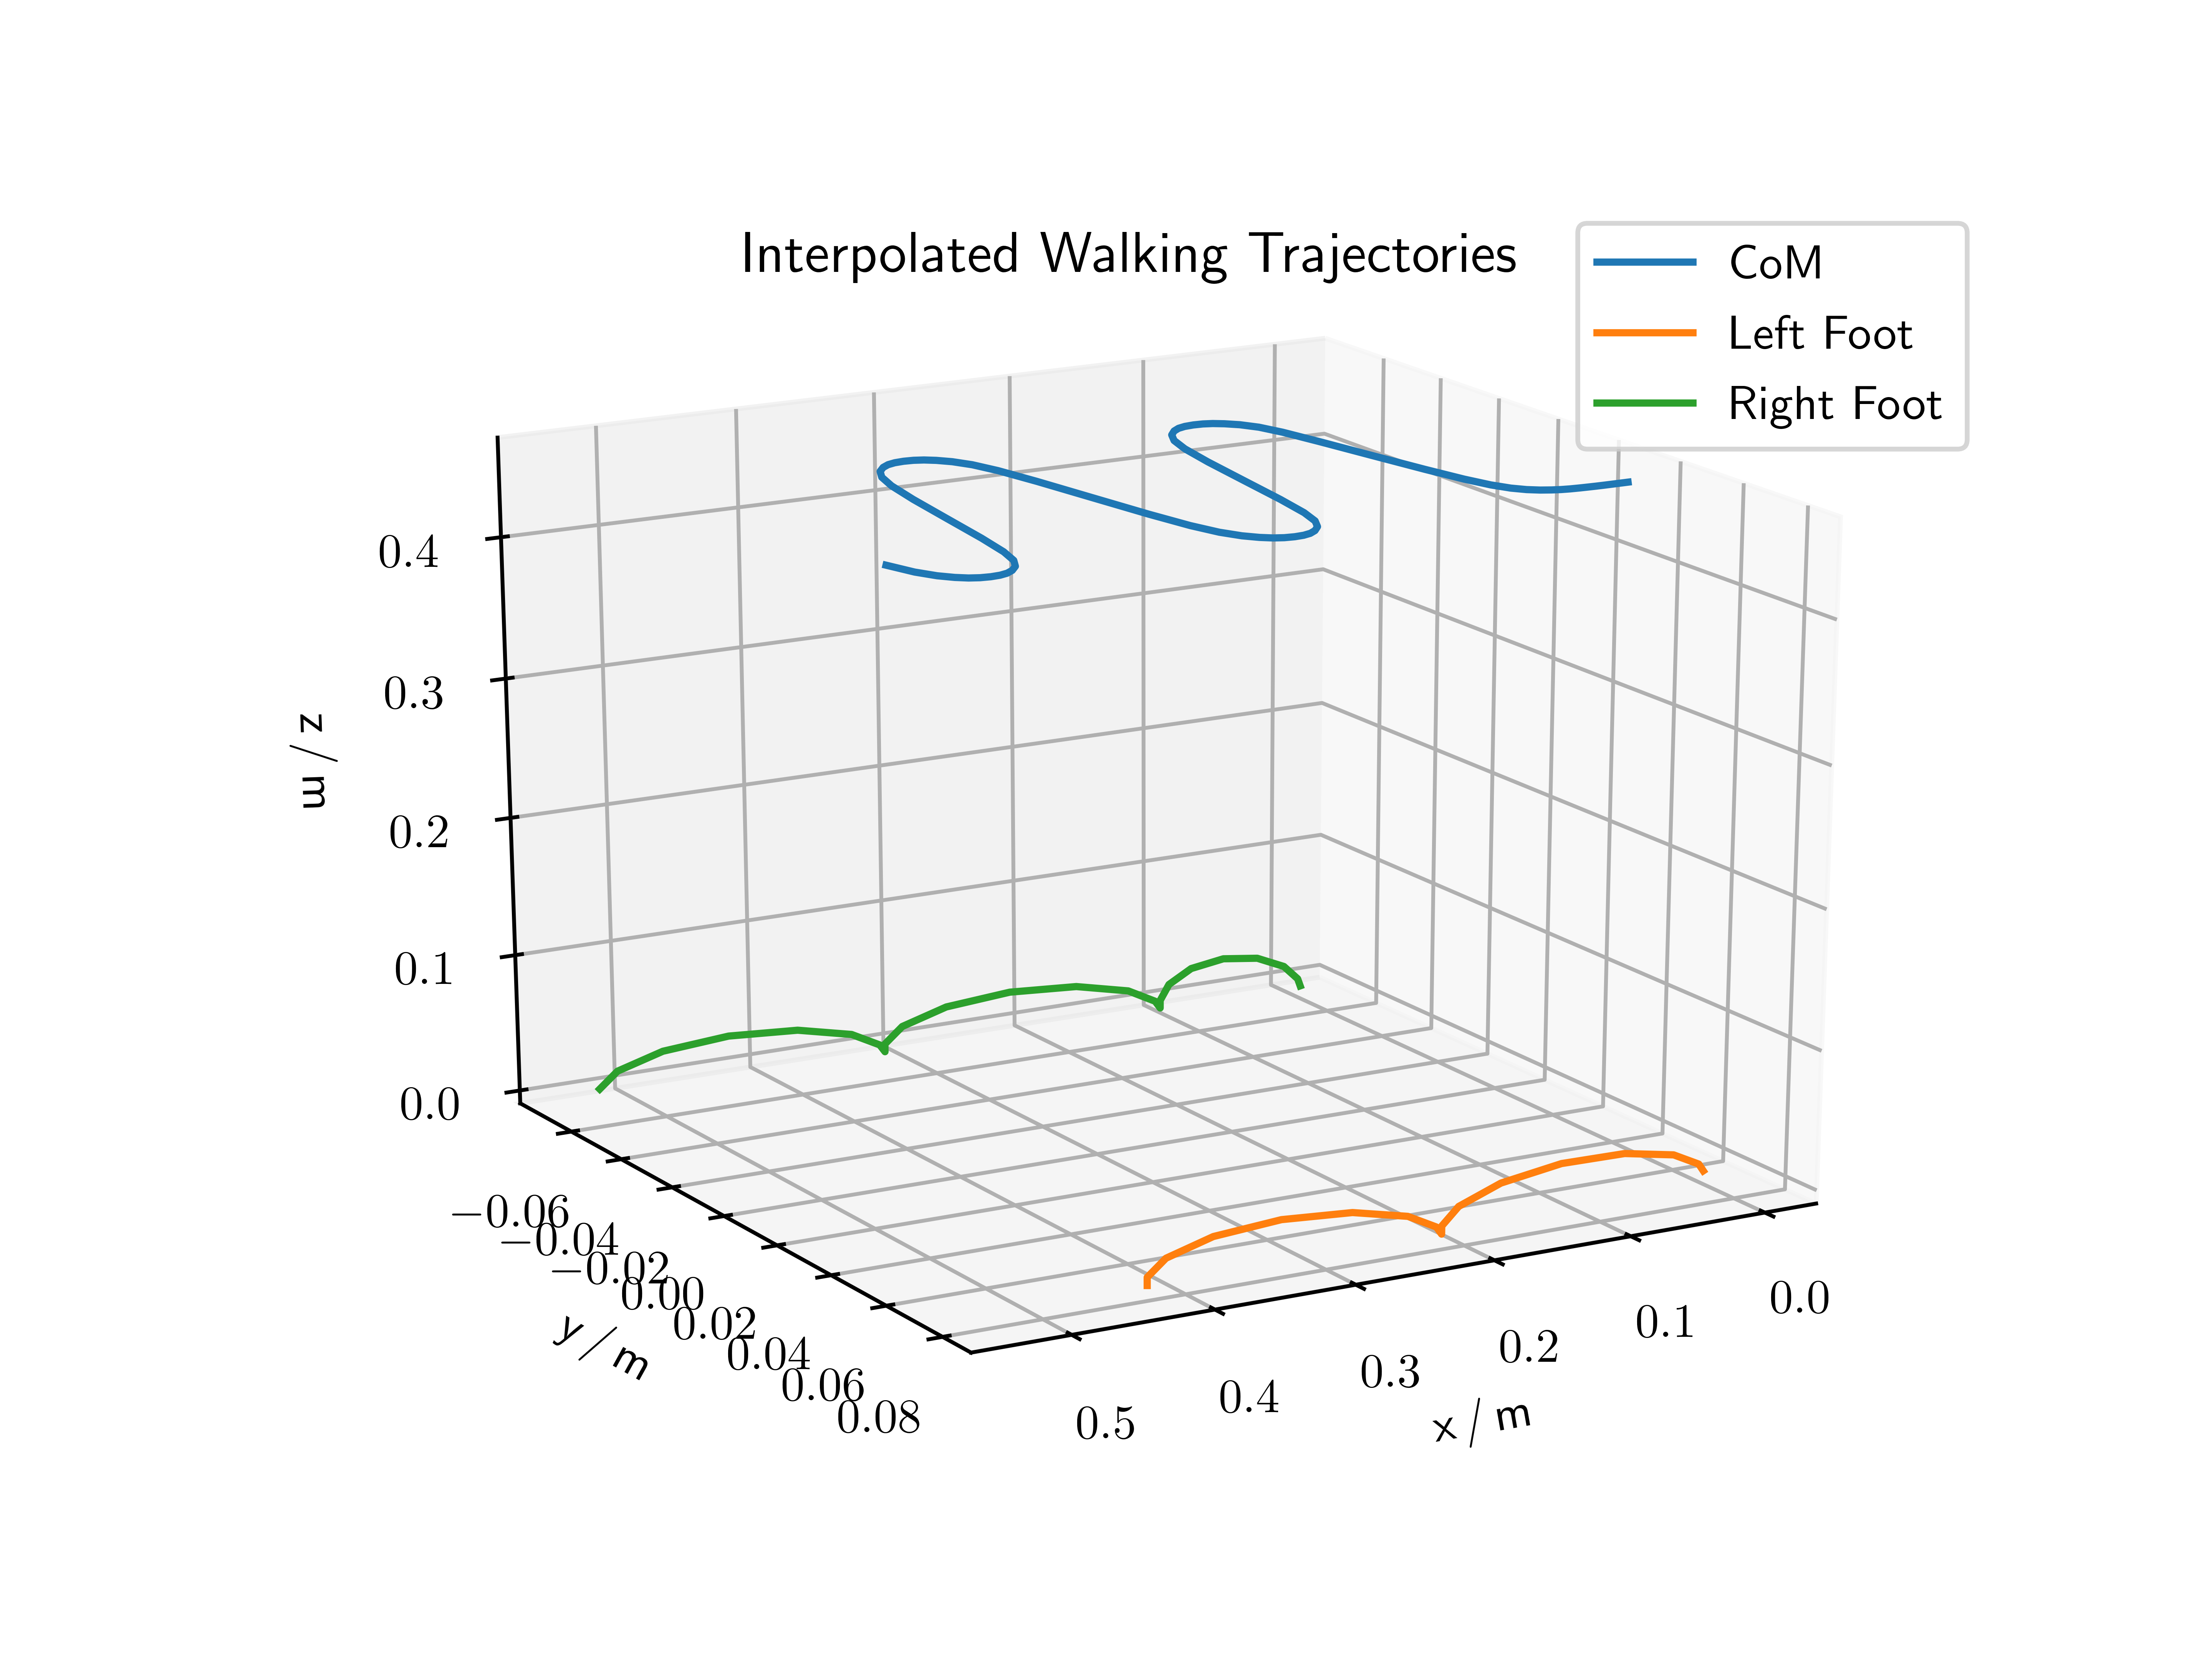
\includegraphics[scale=.4]{chapters/03_background/img/interpolated_results.png}}
	\caption{Uninterpolated trajectories (a), as obtained from the nonlinear model predictive control, and interpolated trajectories (b) for the feet and the center of mass.}
	\label{fig::313_ip}
\end{figure}
\subsubsection{Interpolating the Feet Trajectories}
\begin{align}
	p(t) &= \sum_{i = 0}^{N}a_it^i \\
	\dot{p}(t) &= \sum_{i = 1}^{N}ia_it^{(i-1)} \\
	\ddot{p}(t) &= \sum_{i = 2}^{N}i(i-1)a_it^{(i-2)}
\end{align}
\begin{align}
	z(t = 0) &= z_\text{init} = 0 \\
	\dot{z}(t = 0) &= \dot{z}_\text{init} = 0 \\
	z(t = \frac{T}{2}) &= z_{T/2}\\  
	z(t = T) &= z_\text{end} = 0 \\
	\dot{z}(t = T) &= \dot{z}_\text{end} = 0 
\end{align}
\begin{align}
	\bm{M}\bm{a} &= \bm{c} \\
	\begin{pmatrix}
		1 & 0 & 0              & 0              & 0 \\
		0 & 1 & 0              & 0              & 0 \\
		1 & \left(\frac{T}{2}\right)        & \left(\frac{T}{2}\right)^2  & \left(\frac{T}{2}\right)^3 & \left(\frac{T}{2}\right)^4 \\
		1 & T & T^2            & T^3            & T^4 \\
		0 & 1 & 2T             & 3T^2           & 4T^3 
	\end{pmatrix}
	\begin{pmatrix}
		a_0 \\
		a_1 \\
		a_2 \\
		a_3 \\
		a_4
	\end{pmatrix} &=
	\begin{pmatrix}
		z_\text{init} \\
		\dot{z}_\text{init} \\
		z_{T/2} \\
		z_\text{end}\\
		\dot{z}_\text{end}
	\end{pmatrix}
\end{align}
\begin{align}
	\bm{a}&=\bm{M}^{-1}\bm{c} \\
	\begin{pmatrix}
		a_0 \\
		a_1 \\
		a_2 \\
		a_3 \\
		a_4
	\end{pmatrix} &=
	\begin{pmatrix}
		1 & 0 & 0 & 0 & 0 \\
		0 & 1 & 0 & 0 & 0 \\
		-\frac{11}{T^2} & -\frac{4}{T} & \frac{16}{T^2} & -\frac{5}{T^2} & \frac{1}{T} \\
		\frac{18}{T^3} & \frac{5}{T^2} & -\frac{32}{T^3} & \frac{14}{T^3} & -\frac{3}{T^2} \\
		-\frac{8}{T^4} & -\frac{2}{T^3} & \frac{16}{T^4} & -\frac{8}{T^4} & \frac{2}{T^3}
	\end{pmatrix}
	\begin{pmatrix}
		z_\text{init} \\
		\dot{z}_\text{init} \\
		z_{T/2} \\
		z_\text{end}\\
		\dot{z}_\text{end}
	\end{pmatrix}
\end{align}

\begin{align}
	x(t = 0) &= x_\text{init} \\
	\dot{x}(t=0) &= \dot{x}_\text{init} \\
	\ddot{x}(t=0) &= \ddot{x}_\text{init} \\
	x(t=T) &= x_\text{end}\\
	\dot{x}(t=T) &= \dot{x}_\text{end} \\
	\ddot{x}(t=T) &= \ddot{x}_\text{end} 
\end{align}
\begin{align}
	\bm{M}\bm{a} &= \bm{c} \\
	\begin{pmatrix}
		1 & 0 & 0 & 0 & 0 & 0 \\
		0 & 1 & 0 & 0 & 0 & 0 \\
		0 & 0 & 2 & 0 & 0 & 0 \\
		1 & T & T^2 & T^3 & T^4 & T^5 \\
		0 & 1 & 2 T & 3 T^2 & 4 T^3 & 5 T^4 \\
		0 & 0 & 2 & 6 T & 12 T^2 & 20 T^3
	\end{pmatrix}
	\begin{pmatrix}
		a_0 \\
		a_1 \\
		a_2 \\
		a_3 \\
		a_4 \\
		a_5
	\end{pmatrix} &=
	\begin{pmatrix}
		x_\text{init} \\
		\dot{x}_\text{init} \\
		\ddot{x}_\text{init} \\
		x_\text{end} \\
		\dot{x}_\text{end} \\
		\ddot{x}_\text{end} 
	\end{pmatrix}
\end{align}
\begin{align}
	\bm{a} &= \bm{M}^{-1}\bm{c} \\
	\begin{pmatrix}
		a_0 \\
		a_1 \\
		a_2 \\
		a_3 \\
		a_4 \\
	a_5
	\end{pmatrix} &= 
	\frac{1}{2}
	\begin{pmatrix}
		2 & 0 & 0 & 0 & 0 & 0 \\
		0 & 2 & 0 & 0 & 0 & 0 \\
		0 & 0 & 1 & 0 & 0 & 0 \\
		-\frac{20}{T^3} & -\frac{12}{T^2} & -\frac{3}{T} & \frac{20}{T^3} & -\frac{8}{T^2} & \frac{1}{T} \\
		\frac{30}{T^4} & \frac{16}{T^3} & \frac{3}{T^2} & -\frac{30}{T^4} & \frac{14}{T^3} & -\frac{2}{T^2} \\
		-\frac{12}{T^5} & -\frac{6}{T^4} & -\frac{1}{T^3} & \frac{12}{T^5} & -\frac{6}{T^4} & \frac{1}{T^3} \\
	\end{pmatrix}
	\begin{pmatrix}
		x_\text{init} \\
		\dot{x}_\text{init} \\
		\ddot{x}_\text{init} \\
		x_\text{end} \\
		\dot{x}_\text{end} \\
		\ddot{x}_\text{end} 
	\end{pmatrix}
\end{align}
\subsubsection{Interpolating the Center of Mass Trajectories}